\section{Observations}

\begin{frame}
The DDT(Differential Distribution Table) of SBOX is written below:\\ \\
\begin{center}
\scalebox{0.7}{ 
\begin{tabular}{|c|c|c|c|c|c|c|c|c|c|c|c|c|c|c|c|c|}
\hline
$\Delta_{In}|\Delta_{Out}$ &0&1&2&3&4&5&6&7&8&9&10&11&12&13&14&15 \\
\hline
0&16& 0& 0& 0& 0& 0& 0& 0& 0& 0& 0& 0& 0& 0& 0& 0 \\
\hline
1&0& 0& 0& 4& 2& 0& 2& 0& 2& 0& 0& 2& 0& 0& 2& 2 \\
\hline
2&0& 0& 0& 0& 0& 4& 0& 0& 0& 0& 2& 2& 0& 4& 2& 2 \\
\hline
3&0& 4& 0& 2& 2& 0& 0& 0& 0& 0& 2& 0& 0& 2& 4& 0 \\
\hline
4&0& 2& 0& 2& 2& 0& 2& 0& 0& 2& 0& 2& 0& 2& 0& 2 \\
\hline
5&0& 0& 4& 0& 0& 2& 0& 2& 2& 0& 2& 4& 0& 0& 0& 0 \\
\hline
6&0& 2& 0& 0& 2& 0& 4& 0& 2& 0& 2& 2& 2& 0& 0& 0 \\
\hline
7&0& 0& 0& 0& 0& 2& 0& 2& 2& 2& 0& 0& 2& 0& 4& 2 \\
\hline
8&0& 2& 0& 0& 0& 2& 2& 2& 2& 2& 0& 2& 0& 0& 0& 2 \\
\hline
9&0& 0& 0& 0& 2& 0& 0& 2& 2& 0& 0& 2& 2& 2& 2& 2 \\
\hline
10&0& 0& 2& 2& 0& 2& 2& 0& 0& 0& 4& 0& 2& 0& 2& 0 \\
\hline
11&0& 2& 2& 0& 2& 4& 2& 0& 2& 2& 0& 0& 0& 0& 0& 0 \\
\hline
12&0& 0& 0& 0& 0& 0& 2& 2& 0& 2& 2& 0& 4& 2& 0& 2 \\
\hline
13&0& 0& 4& 2& 2& 0& 0& 0& 0& 2& 0& 0& 2& 2& 0& 2 \\
\hline
14&0& 2& 2& 4& 0& 0& 0& 4& 0& 2& 2& 0& 0& 0& 0& 0 \\
\hline
15&0& 2& 2& 0& 2& 0& 0& 2& 2& 2& 0& 0& 2& 2& 0& 0 \\
\hline
\end{tabular}
}
 \end{center}
 The maximum differential probability is KLEIN's SBOX is 4/16 i.e 1/4 and some of the transitions leading to it are $(\Delta_{In},\Delta_{Out})$= (1,4),(3,1) etc.\\
\end{frame}

\begin{frame}{Attacks on KLEIN cipher}
\textbf{Round Reduced Attack}\\
The weakness present in the Rotate Nibbles and Mix columns step is exploited here in this attack.\\
Firstly, a 6 round truncated differential distinguisher with $2^{-29}$ is made.Using this as base, an 8 Round distinguisher is constructed.One of the assumption is they will be having access to round wise outputs.\\
Lets have look at few terminologies used in this attack:\\
\begin{enumerate}
    \item $X_{i}$ : The input of the i-th round.
    \item $\Delta X_{i}$ : The input difference of the i-th round.
    \item $Y_{i}$ : The input of SubNibbles in the i-th round .
    \item $\Delta Y_{i}$ : The input difference of SubNibbles in the i-th round .
    \item $X_{i,j}$ : The j-th nibble of the $X_{i}$ , where j = 0, 1, ...15.
    \item $sk_{i}$ : The subkey of the i-th round.
    \item $X || Y$ : The the concatenation of X and Y.
\end{enumerate}
\end{frame}

\begin{frame}
The state of encryption: \\
\begin{center}
\begin{tabular}{|c|c|c|c|}
\hline
0&4&8&12\\
\hline
1&5&9&13\\
\hline
2&6&10&14 \\
\hline
3&7&11&15\\  
\hline
\end{tabular}
\end{center}
The number in box represents the Nibble numbers of the 64 bit data block.
\textbf{Some properties and observations of KLEIN cipher}\\
\textbf{Lemma1.} If a byte is of the form $0z$, where $z$ is a 4-bit string
with MSB bit as 0, then $0z$ multiply by $x$ is equal to $0z^{'}$, where $z ^{'}$
is a 4-bit string.\\
The following observations are derived based on above lemma.\\ \\

\end{frame}

\begin{frame}
    \textbf{Observation 1.} 
\begin{math}
\begin{bmatrix}
2&3&1&1\\
1&2&3&1\\
1&1&2&3\\
3&1&1&2
\end{bmatrix}
\text{x}
\begin{bmatrix}
0z \\
00 \\
00 \\
00 
\end{bmatrix} = 
\begin{bmatrix}
0z^{'}_{1} \\
0z^{'}_{2} \\
0z^{'}_{3} \\
0z^{'}_{4} 
\end{bmatrix}
\end{math} if only if MSB $z$ is 0. \\ \\
\textbf{Observation 2.} 
\begin{math}
\begin{bmatrix}
2&3&1&1\\
1&2&3&1\\
1&1&2&3\\
3&1&1&2
\end{bmatrix}
\text{x}
\begin{bmatrix}
00 \\
00 \\
0z_{1} \\
0z_{2} 
\end{bmatrix} = 
\begin{bmatrix}
0z^{'}_{1} \\
0z^{'}_{2} \\
0z^{'}_{3} \\
0z^{'}_{4} 
\end{bmatrix}
\end{math} if only if MSB $z_{1}$ and $z_{2}$ is 0. \\ \\
\textbf{Observation 3}
\begin{math}
\begin{bmatrix}
2&3&1&1\\
1&2&3&1\\
1&1&2&3\\
3&1&1&2
\end{bmatrix}
\text{x}
\begin{bmatrix}
0z_{1} \\
0z_{2} \\
0z_{3} \\
0z_{4} 
\end{bmatrix} = 
\begin{bmatrix}
0z^{'}_{1} \\
0z^{'}_{2} \\
0z^{'}_{3} \\
0z^{'}_{4} 
\end{bmatrix}
\end{math}
 if only if MSB's of $z_{1},
z_{2} ,
z_{3} \;and\;
z_{4} $ are 0.\\
\end{frame}
\begin{frame}{Truncated Six Round Differential Distinguisher}
Based on the above observations, we show that if the input difference of 6-round KLEIN are all zero except the 13-th nibble, after encryption, the first and the third column of state matrix will stay 0 with the probability of $2^{-29}$.\\
This happens because the difference in column will not transfer to other column due to the RotateBits algorithm and above observations. \\ This is the reason for high probability 6-round differential distinguisher.
\end{frame}
\begin{frame}

\begin{figure}[h!]
    \centering
    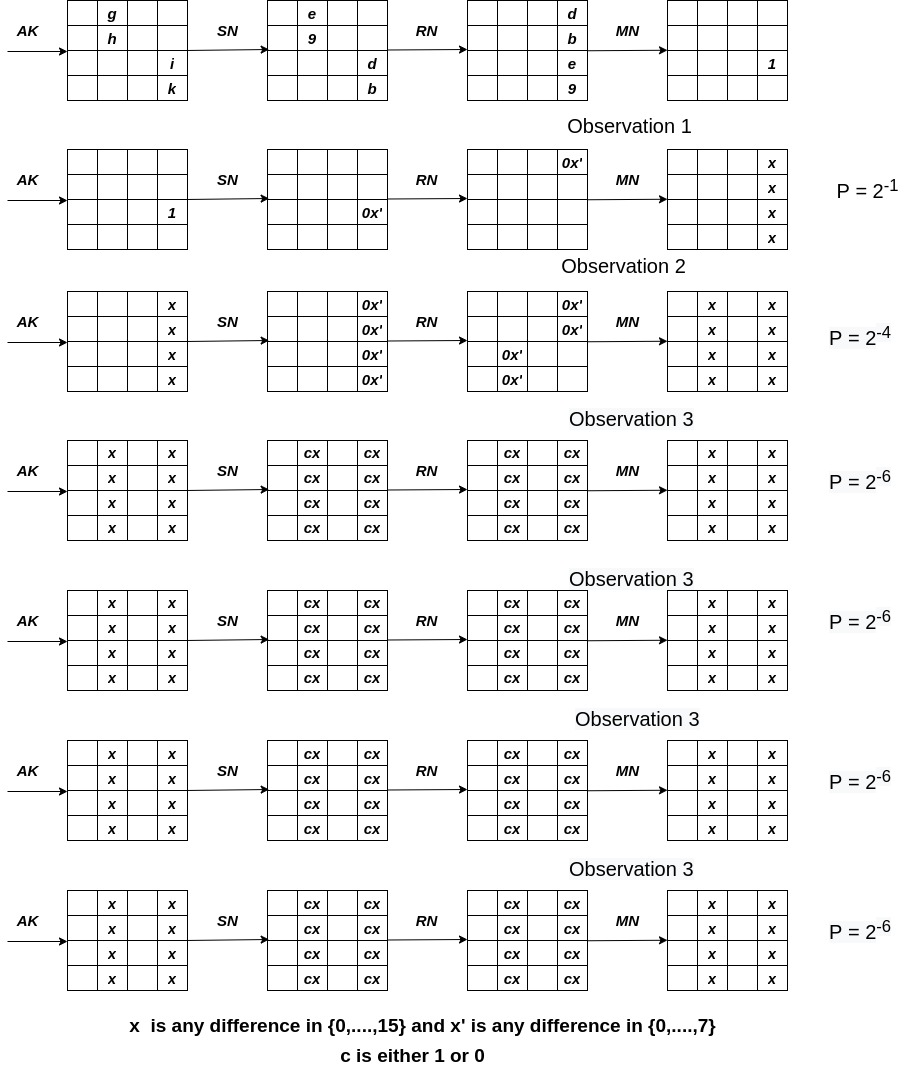
\includegraphics[width= 8cm, height= 8cm, keepaspectratio]{images/7round characteristic of round reduced.jpg}
    \caption{7 round characteristic of 8 Round Distinguisher}
    \label{fig:6distinguisher}
\end{figure}
\\ \\
\end{frame}

\begin{frame}{Truncated Differential Analysis of 8-Round KLEIN-64}
The 8 round distinguisher is constructed by adding an extra layer at the top and bottom of the 6 round distinguisher.\\
As this is CPA(chosen plain text) attack, we choose plain text pairs such a way that input difference to the second round is all zero except the 13-th nibble. We actually obtain the required input pairs of first round by reverse tracing the single nibble that should be active at the end of the round.This process is also diplayed in Figure \ref{fig:6distinguisher} \\
\end{frame}
\begin{frame}
\textbf{ The Steps and Analysis Procedure}\\ \\
\textbf{Step1.} We will choose the input plaintexts in such a way that, all nibbles have some fixed values except four nibbles $X_{1,1} , X_{1,3} , X_{1,13} , X_{1,15}$. If we fix the values and change the values only in these 4 nibbles, that is called one structure. There are $2^{16}$ possible plain texts in one structure.\\
We can form nC2 i.e $(2^{16} \text{x} (2^{16} - 1))/2 = 2^{31}$ plain text pairs from those $2^{16} $ plain texts.\\ If we took m structures then we will have $2^{16}m$ plain texts and $2^{31}m$ pairs.\\ \\ \\ \\
\textbf{Step 2.} By Guessing the values(trying all possible values)  of the subkey nibbles $sk_{1,1} , sk_{1,3} , sk_{1,13} , sk_{1,15}$ we should make sure that $\Delta SubNibbles(X_{1,1} \oplus sk_{1,1} ) = 0e, \Delta SubNibbles(X_{1,3} \oplus sk_{1,3} ) = 09, \Delta SubNibbles(X_{1,13} \oplus sk_{1,13} ) =
0d\; and \;\Delta S(X_{1,15} \oplus sk_{1,15} ) = 0b.$ The probability of this is $2^{-16}$ as we are fixing values of 4 particular nibbles, so the expected number of confirming pairs is $2^{31} \;\text{x}\; m\; \text{x} \;2^{-16} = 2^{15} m$. 

\end{frame}
\begin{frame}
\textbf{Step 3.} Now take those remaining $2^{15}m$ pairs and encrypt them upto 8 rounds. Then verify the third and first columns output difference of $MC^{-1}$  to zero. If not, discard the key guess. The probability of this event to happen is $(2 ^{-16})^{2}$ so the number of confirming pairs would be $2^{15} \;*\; m \;*\; (2 ^{-16})^{2} = 2^{-17}m$. Now we should use meet in the middle technique. \\ \\ \\
\textbf{Step 4}. For the obtained confirming pairs from previous step,  guess the value of the subkey $sk_{9,j}$, j = 0, 1, \ldots, 7 to inverse the SubNibbles step and find input difference of 8-th round, i.e $\Delta X_{8,j}$ , j = 0, 1, \ldots, 7. \\ \\
\end{frame}

\begin{frame}
    \textbf{Step 5.} Now, reverse the MixColumns step i.e $MC^{-1}$ on $\Delta X_{8}$ and verify whether the first column difference is zero and also the MSB of second column should be all 1 or all 0. If it failed to satisfy the above condition then discard the key guess.The expected confirming pairs is $2^{17}\;*\;m\;*\;2^{-7} = 2^{-24}m$ as the probability of the above event is $2^{-7}$.\\ \\ \\
\textbf{Step 6.} Guess the remaining 16 bits key in the similar way by verifying third and fourth columns.\\ \\ \\
\textbf{Time and Space Complexity} \\
Step 2 takes $2^{16}*2^{16}/8$ one round 64 bit encryptions. In Step 3 it takes $2^{15}*2^{16}*2^{16}*7/8$ encryptions whereas in step 4 it takes $2^{-17}*2^{16}*2^{16}*2^{32}/8$ encryptions are required and step 6 takes about $2^{16}$ encryptions.So overall time complexity $2^{46.8}$ one round 64 bit encryptions.The data complexity is $2^{32}$ plaintexts. Memory complexity is $2^{32}$ 64bit states. 
\end{frame}

\begin{frame}{Integral Analysis}
	\textbf{Observations}
	\begin{enumerate}
		
		\item If we give $2^{32}$ different input values to the Rotate Nibble then after the Rotate Nibble and sub nibble operation and 3 rounds of KLIEN all the output nibbles are balanced \\ \\
		
		\item If in the input state $i_{th}$ nibble is active where i=0,1,2,3,12,13,14,15 then after 1 round of KLIEN and one add key and one sub nibble all $j_{th}$ nibbles are active where j=8,9,10,11,12,13,14,15 \\
		\begin{tabular}{|c|c|c|c|c|c|c|c|}
			\hline
			A & A & C & A & C & C & C & C \\
			\hline
			C & C & C & C & A & A & A & A\\
			\hline
		\end{tabular}
		$\xrightarrow{1.5round}$
		\begin{tabular}{|c|c|c|c|c|c|c|c|}
			\hline
			X & X & X & X & X & X & X & X \\
			\hline
			A & A & A & A & A & A & A & A\\
			\hline
		\end{tabular}\\
	\end{enumerate}
\end{frame}
\begin{frame}
	\textbf{Combining Obs. to Get 5 round Distinguisher}\\
	\begin{tabular}{|c|c|c|c|c|c|c|c|}
		\hline
		A & A & C & A & C & C & C & C \\
		\hline
		C & C & C & C & A & A & A & A\\
		\hline
	\end{tabular}\\
	\begin{center}$\downarrow 5 round$\\ \end{center}
	\begin{tabular}{|c|c|c|c|c|c|c|c|}
		\hline
		B & B & B & B & B & B & B & B \\
		\hline
		B & B & B & B & B & B & B & B\\
		\hline
	\end{tabular}
\end{frame}

\begin{frame}{ 7 round integral attack}
	
	\begin{itemize}
	\item We can take our 5 round distinguisher one step further as Round key addition does not change the Balance property. Let $Y_{j}$ be the input to 6th round Sbox of the  plaintext where j denotes the jth nibble. Then the xor sum of $Y_{j}$ over all plaintext is 0 \\
	
	\\
	Let $y_{j}$ be the jth nibble obtained after Reversing the sub bytes.\\ \\ Clearly $y_{j}$=$S^{-1}$ ($X_{j}\oplus sk_{7,j}) $ 
	\\ \\
	\item After Mix columns of 6th round we get the following relation \\ \\
	$Y_{4}||Y_{5}$ = $S^{-1}(R^{-1}(e.(y_{1}||y_{2})\oplus b.(y_{2}||y_{3})\oplus d.(y_{4}||y_{5})\oplus9.(y_{6}|| y_{7}))
	\oplus sk_{6,4} || sk_{6,5})$
	\\ \\
	\end{itemize}
\end{frame}
\begin{frame}
	\textbf{Analysis Procedure}
	\begin{itemize}
		\item We first get \textbf{5} sets of $2^{32}$ plaintexts. For each of these sets we do the following-
		\item Guess $sk_{7,0}$,$sk_{7,1}$,$sk_{7,2}$,$sk_{7,3}$ for each plaintext and obtain $e.(y_{1}||y_{2})\oplus b.(y_{2}||y_{3})$\\
		Let $u1$=$e.(y_{1}||y_{2})\oplus b.(y_{2}||y_{3})$ \\.
		Now we get $2^{24}$ different values of $(u1\oplus d.(y_{4}||y_{5})\oplus9.(y_{6}|| y_{7}))$ as each of the term is 8 bytes.
		
		\item Guess $sk_{7,4}$,$sk_{7,5}$ and obtain 
		$d.(y_{4}||y_{5})$\\
		Let $u2$=$u1 \oplus (y_{4}||y_{5})$  \\  
		Now are left with $2^{16}$ values of $(u2\oplus9.(y_{6}|| y_{7}))$ \\
	\end{itemize}
\end{frame}
\begin{frame}
	\begin{itemize}
	
		\item Guess $sk_{7,6}$,$sk_{7,7}$ and obtain 
		$d.(y_{6}||y_{7})$\\
		Let $u3$=$u2 \oplus (y_{6}||y_{7})$  \\  
		Now are left with $2^8$ values of $(u3)$ \\
		\item Now our equation becomes \\
		$Y_{4}||Y_{5}$ = $S^{-1}(R^{-1}(u3)
		\oplus sk_{6,4} || sk_{6,5})$\\
		\item We now guess $sk_{6,4}$ and $sk_{6,5}$ and then obtain the Sum of $Y_{4}||Y_{5}$. If its not 0 we discard our guess. Wrong key can also give 0  with 1/128 probability and therefore we used 5 sets
	\end{itemize}
\end{frame}